% AMPERE POINT — projekt uniwersalnego słupka ładowania AP-S1 + zestaw doposażenia AP-R1
% kompilacja: xelatex
\documentclass[11pt,a4paper]{article}
\usepackage{fontspec}
\setmainfont{DejaVu Serif}
\setsansfont{DejaVu Sans}
\usepackage{amssymb}
\usepackage{xcolor}
\definecolor{apnavy}{RGB}{16,42,84}
\definecolor{apred}{RGB}{200,30,40}
\definecolor{apgray}{RGB}{120,126,133}
\usepackage[margin=2.0cm]{geometry}
\usepackage{tikz}
\usetikzlibrary{patterns}
\usepackage{booktabs}
\usepackage{longtable}
\usepackage{enumitem}
\usepackage{titlesec}
\usepackage{parskip}
\usepackage[colorlinks=true,linkcolor=apnavy,urlcolor=apnavy]{hyperref}
\renewcommand{\contentsname}{Spis treści}
\renewcommand{\tablename}{Tabela}
\renewcommand{\figurename}{Rys.}
\hyphenpenalty=3000 \tolerance=2000 \emergencystretch=2em
\titleformat{\section}{\large\bfseries\color{apnavy}}{\thesection.}{0.6em}{}
\titleformat{\subsection}{\normalsize\bfseries\color{apnavy}}{\thesubsection.}{0.6em}{}
\setlist{nosep,leftmargin=1.4em}

% strzałka wymiarowa pozioma: \dimh{x1}{x2}{y}{etykieta}
\newcommand{\dimh}[4]{\draw[<->,thin] (#1,#3) -- (#2,#3) node[midway,fill=white,inner sep=1pt,font=\scriptsize]{#4};}
% strzałka wymiarowa pionowa: \dimv{x}{y1}{y2}{etykieta}
\newcommand{\dimv}[4]{\draw[<->,thin] (#1,#2) -- (#1,#3) node[midway,fill=white,inner sep=1pt,font=\scriptsize]{#4};}

\title{\textbf{\color{apnavy}AMPERE POINT}\\[4pt]
\large Uniwersalny słupek ładowania AP-S1 z zadaszeniem\\[2pt]
\normalsize projekt koncepcyjny z rysunkami wymiarowymi + zestaw doposażenia AP-R1 dla obecnych słupków\\
wersja 1}
\author{Opracowanie wewnętrzne AMPERE POINT}
\date{12 lipca 2026}

\begin{document}
\maketitle
\vspace{-1.4em}

\noindent\textbf{Cel dokumentu.} Projekt nowego, uniwersalnego słupka pod ładowarki AMPERE POINT
(wallbox serii Prime albo ładowarka przenośna Q11) wraz z gniazdami, zgodny z trzema wymaganiami:
\textbf{(1)} słupek ma być zadaszony, \textbf{(2)} kable mają wchodzić z ziemi i biec wewnątrz słupka,
\textbf{(3)} gniazda mają się przykręcać łatwo, bez wiercenia w metalu. Dokument zawiera analizę
stanu obecnego, przegląd produktów konkurencji (stan cen: lipiec 2026), koncepcję konstrukcji,
rysunki wymiarowe i listę materiałów. Uzupełnieniem jest interaktywna wizualizacja 3D w pliku
\texttt{AMPERE\_POINT\_slupki\_3D\_v1.html}. Rysunki są koncepcyjne --- to podstawa do rozmowy
z wykonawcą stali i do wykonania dokumentacji produkcyjnej (pliki DXF, czyli wektorowe pliki
do cięcia laserowego), nie gotowa dokumentacja warsztatowa.

\tableofcontents

\section{Stan obecny i wnioski ze zdjęć}
Na zdjęciach z folderu \texttt{slupki} widać dwie konfiguracje na tym samym typie słupka
(czarny profil zamknięty na płycie podstawy z otworami na kotwy):

\textbf{Konfiguracja 1: wallbox + gniazdo siłowe.} Wallbox wisi na wsporniku przykręconym do
profilu, a obok --- na blaszanym kątowniku --- przykręcone jest natynkowe gniazdo siłowe
(gniazdo pięciobiegunowe 400~V wg normy PN-EN 60309, potocznie ,,siła''; na zdjęciu iLuve, IP44).
Wallbox jest zakończony wtyczką siłową wpinaną w to gniazdo.

\textbf{Konfiguracja 2: ładowarka Q11 + gniazdo Schuko.} Q11 siedzi w uchwycie na froncie słupka,
niżej przykręcone jest szare gniazdo jednofazowe z klapką (gniazdo typu Schuko --- zwykłe gniazdo
230~V z bolcami ochronnymi po bokach; na zdjęciu Dr.~Storm z oferty AMPERE POINT), a wtyczka
siłowa Q11 zwisa z tyłu. Pod spodem uchwyt na wtyczkę Typ~2 (złącze ładowania samochodu).

Problemy wspólne dla obu konfiguracji:
\begin{itemize}
\item \textbf{każdy montaż gniazda = wiercenie w profilu} (widoczne wkręty do blachy) --- pracochłonne,
niszczy powłokę lakierniczą (ognisko korozji), a otwory są nie do cofnięcia przy zmianie konfiguracji;
\item \textbf{kable biegną po zewnętrzu} --- pętle przewodów przy podstawie i wzdłuż profilu wyglądają
prowizorycznie, są narażone na promieniowanie słoneczne (UV degraduje izolację), zaczepienie nogą
i wandalizm;
\item \textbf{brak jakiejkolwiek osłony od deszczu i śniegu} nad ładowarką, gniazdami i wtyczkami;
\item \textbf{brak miejsca na zabezpieczenia} --- wyłącznik różnicowoprądowy i nadprądowy muszą być
w rozdzielnicy budynku, daleko od stanowiska;
\item wnętrze profilu jest niewykorzystane, choć to naturalny kanał kablowy.
\end{itemize}

\section{Konkurencja --- co oferuje rynek (lipiec 2026)}
\label{sec:konkurencja}
Przegląd objął polskich i europejskich producentów słupków (stojaków) pod ładowarki AC oraz
zintegrowane stacje słupkowe. Szczegóły i źródła w tabeli~\ref{tab:konkurencja} i na końcu dokumentu.

\begin{table}[h]\small
\caption{Porównanie słupków dostępnych na rynku (ceny brutto, stan: lipiec 2026).}
\label{tab:konkurencja}
\begin{tabular}{p{3.4cm}p{1.9cm}p{1.2cm}p{1.6cm}p{2.0cm}p{1.8cm}p{2.2cm}}
\toprule
Produkt & Cena & Daszek & Kabel w~środku & Gniazda 230/400~V & Montaż bez wiercenia & Miejsce na zabezpieczenia\\
\midrule
\textbf{AP-S1 (ten projekt)} & 999--1199~zł (propozycja) & \textbf{tak} & \textbf{tak} & \textbf{tak, na płytach} & \textbf{tak, raster} & \textbf{tak, szyna TH35}\\
Platinet uniwersalny z daszkiem & 1100~zł & tak & tak & nie & częściowo (adapter) & nie\\
Green Cell GC EV Stand & ok.~480~zł & nie & tak & nie & nie (dedykowany) & nie\\
Green Wallbox (8 modeli) & 649--979~zł & nie & tak & nie & nie (dedykowane) & nie\\
Wallbox Eiffel Basic & ok.~450--550~USD & opcja +80~USD & tak & nie & nie (Pulsar) & nie\\
Enelion Vertica & moduły 5000--6650~zł & nie & tak & nie & --- (stacja zintegrowana) & tak\\
Tuneon (DE), stele & 147--165~EUR & opcja & tak & nie & nie (dedykowane) & nie\\
AMP-BOX ze słupkiem (oferta własna) & 999~zł & nie dot. (szafa) & tak & do samodzielnego montażu & nie & tak (miejsce w szafie)\\
\bottomrule
\end{tabular}
\end{table}

Wnioski z przeglądu:
\begin{itemize}
\item \textbf{Segment 500--1100~zł to gięte słupki bez gniazd.} Green Wallbox i Green Cell sprzedają
słupki dedykowane pod konkretne modele wallboxów; uniwersalność deklaruje tylko Platinet (adapter
aluminiowy z rastrem otworów) --- i tylko Platinet ma daszek w standardzie.
\item \textbf{Nikt w tym segmencie nie przewiduje gniazd 230/400~V na słupku} --- a to dokładnie
model sprzedaży AMPERE POINT (ładowarka przenośna + gniazdo). Klient konkurencji, który chce gniazdo
przy stanowisku, musi wiercić samodzielnie --- czyli dokładnie problem, który mamy dziś.
\item \textbf{Miejsce na zabezpieczenia przy stanowisku ma tylko segment premium} (Enelion Vertica ---
zintegrowana stacja za kilkanaście tysięcy złotych za komplet). W segmencie do 1500~zł nikt tego nie daje.
\item \textbf{Fundament prefabrykowany jako akcesorium} sprzedaje Green Wallbox (399~zł) --- dobry
wzorzec do skopiowania, bo skraca montaż u klienta.
\item Wallbox Eiffel pokazuje, że daszek bywa sprzedawany jako \textbf{płatna opcja} (ok.~80~USD) ---
u nas będzie w standardzie, co jest łatwym argumentem sprzedażowym.
\end{itemize}

\section{Synergia z ofertą AMPERE POINT}
Nowy słupek nie powstaje w próżni --- sklep \texttt{amperepoint.pl} ma już komponenty, które projekt
wykorzystuje wprost:
\begin{itemize}
\item \textbf{Prime Wallbox 11/22~kW z wtyczką} --- urządzenie do konfiguracji A (montaż na płycie
uniwersalnej);
\item \textbf{Q11 / seria Q z wtyczką siłową 16~A} --- urządzenie do konfiguracji B (istniejący uchwyt);
\item \textbf{Dr.~Storm} --- opancerzone gniazdo zewnętrzne 16~A/IP55 z głowicą regulowaną o 90 stopni
i blokadą na kłódkę; idealne jako gniazdo Schuko na słupku (płyta P3);
\item \textbf{uchwyt wtyczki Typ~2 AMPERE POINT} --- widoczny już na zdjęciach obecnych słupków;
\item \textbf{AMP-BOX} --- zamykana szafa na słupku; pozostaje w ofercie jako wariant ,,ładowarka pod
kluczem'', AP-S1 jest wariantem otwartym, tańszym wizualnie i smuklejszym;
\item \textbf{kable Typ~2 Power Mamba} --- naturalny element zestawów sprzedażowych.
\end{itemize}
Styl marki do zachowania w konstrukcji: czarny mat jako kolor bazowy, srebrny akcent poziomy
(jak pas na obudowie Q11), czerwone logo. Ton komunikacji produktowej AMPERE POINT (nazwy w rodzaju
,,Dr.~Storm'', ,,Power Mamba'') dopuszcza chwytliwą nazwę handlową --- propozycja: \textbf{,,Ampere
Tower''} dla AP-S1 i \textbf{,,Tower Kit''} dla zestawu doposażenia AP-R1 (oznaczenia AP-S1/AP-R1
pozostają jako techniczne).

\section{Koncepcja słupka AP-S1}
\subsection{Architektura}
Jedna wspólna platforma mechaniczna, konfigurowana płytami adapterowymi (rys.~\ref{fig:front},
\ref{fig:bok}, \ref{fig:przekroj}):
\begin{itemize}
\item \textbf{Korpus}: słup o przekroju prostokątnym $200\times120$~mm z blachy stalowej 3~mm, gięty
z dwóch ceowników (profili o przekroju w kształcie litery C) łączonych wzdłużnie, wysokość 1350~mm;
u dołu przyspawany do płyty podstawy $300\times250\times8$~mm. Wysokość całkowita z daszkiem: 1455~mm.
\item \textbf{Daszek}: blacha 2~mm gięta w jednym kawałku, rzut $400\times350$~mm, spadek $12^\circ$
do tyłu, obrzeża zagięte 15~mm w dół; wysunięcie 230~mm przed lico frontu osłania wallbox/Q11
i gniazda; przykręcany czterema śrubami M6 do nitonakrętek (nitonakrętka: tulejka z gwintem
zaciskana fabrycznie w blasze --- daje gwint w cienkiej ściance bez spawania) w górnej ściance korpusu.
Kolor srebrny (RAL~9006) --- akcent stylu marki.
\item \textbf{Raster montażowy} (kluczowa innowacja): na froncie i na tylnej ścianie dwa pionowe pasy
\textbf{kwadratowych otworów $9{,}5\times9{,}5$~mm w podziałce 25~mm}, rozstaw pasów 140~mm, w strefie
500--1300~mm nad gruntem. To ten sam system, co w szafach teleinformatycznych: w kwadratowy otwór
wpina się od wewnątrz \textbf{nakrętkę koszykową M6} (nakrętka w sprężystym koszyczku blaszanym)
i przykręca dowolny osprzęt śrubą M6 --- \textbf{zero wiercenia, pełna odwracalność, dowolna wysokość
co 25~mm}. Na bokach pojedynczy pas otworów co 50~mm (strefa 700--1200~mm) na uchwyty kabla.
\item \textbf{Płyty adapterowe} (blacha 3~mm, proszkowana, w komplecie dławik --- czyli szczelny
przepust kablowy z gwintem --- i uszczelka): P1 --- uniwersalna pod wallbox $300\times300$~mm z siatką
otworów $\varnothing$5{,}5 co 20~mm; P2 --- pod gniazdo siłowe 16/32~A; P3 --- pod Dr.~Storm/Schuko;
P4 --- pod uchwyt Q11; P5 --- pod uchwyt wtyczki Typ~2; P6 --- zaślepka. Za każdą pozycją płyty
w korpusie jest fabryczny otwór rewizyjny $120\times250$~mm --- po odkręceniu płyty jest dostęp ręką
do wnętrza (podłączenie gniazda bez demontażu słupka).
\item \textbf{Kable}: wchodzą z ziemi przez centralny otwór owalny $80\times60$~mm w płycie podstawy
(przepust membranowy z gumy EPDM) i biegną kanałem wewnętrznym do gniazd i ładowarki. Żadnego kabla
na zewnątrz.
\item \textbf{Strefa zabezpieczeń}: wewnątrz, na wysokości ok.~600~mm, szyna TH35 (znormalizowana
szyna 35~mm do aparatów elektrycznych) długości 160~mm + złączki N/PE. Mieści wyłącznik
różnicowoprądowy i nadprądowy (do 8 modułów) albo licznik energii. Dostęp przez dolny otwór rewizyjny.
Opcjonalnie zamiast aparatów na szynie --- mała rozdzielnica natynkowa IP65.
\item \textbf{Uziemienie}: śruba M8 z oznaczeniem PE przy podstawie; daszek i płyty adapterowe
połączone linkami wyrównawczymi (ciągłość połączeń ochronnych części metalowych).
\item \textbf{Wersja DUO}: tylny raster jest identyczny jak przedni, więc drugi komplet
(wallbox/Q11 + gniazda) montuje się plecami do siebie --- jeden słupek, dwa stanowiska.
\item \textbf{Wykończenie}: ocynk + lakier proszkowy RAL~9005 mat strukturalny (korpus), RAL~9006
(daszek), logo AmperePoint czerwone na froncie pod daszkiem. Masa ok.~30~kg.
\item \textbf{Opcja}: listwa LED 12~V IP65 pod daszkiem (zasilacz na szynie TH35) --- oświetlenie
stanowiska i efekt ,,premium'' po zmroku.
\end{itemize}

\subsection{Konfiguracje}
\textbf{A --- wallbox:} P1 z wallboxem Prime (środek na 1250~mm), P2 z gniazdem siłowym na 950~mm
(wtyczka wallboxa wpięta pod daszkiem), P5 z uchwytem Typ~2 na boku (850~mm).\\
\textbf{B --- Q11:} P4 z uchwytem Q11 na górze (1250~mm), P2 z gniazdem siłowym 16~A na 950~mm
(krótki kabel Q11 wpięty na stałe, schowany za słupkiem), P3 z Dr.~Storm na 1000~mm z boku lub
z tyłu (dla ładowarek jednofazowych klienta), P5 jak wyżej.\\
Wysokości gniazd mieszczą się w wymaganym normami przedziale 0{,}5--1{,}5~m nad poziomem stanowiska
(HD~60364-7-722 dla obwodów zasilania pojazdów; gniazda wg PN-EN 60309 i osprzęt min.~IP44).

\subsection{Posadowienie --- trzy warianty}
\begin{enumerate}
\item \textbf{Kotwy do betonu}: 4 kotwy wklejane M12$\times$160 w istniejącą płytę/kostkę na podbudowie
betonowej; rozstaw otworów $240\times190$~mm (rys.~\ref{fig:podstawa}).
\item \textbf{Fundament prefabrykowany} (akcesorium, wzorem konkurencji): blok betonowy
$300\times300\times800$~mm z zabetonowaną rurą osłonową $\varnothing$50 wyprowadzoną w osi otworu
kablowego i 4 szpilkami M12; wykop, wstawienie, obsypanie --- bez betonowania na mokro.
\item \textbf{Fundament wkręcany} (innowacja w tej klasie produktu): śruba ziemna $\varnothing$76,
długość 865~mm, z płytą adapterową pod rozstaw $240\times190$~mm; montaż w 30~minut bez betonu,
pełna odwracalność --- ważne dla klientów wynajmujących nieruchomość.
\end{enumerate}

\section{Rysunki wymiarowe}
Wszystkie wymiary w milimetrach. Skala poglądowa; do produkcji powstaną pliki DXF.

\begin{figure}[h]\centering
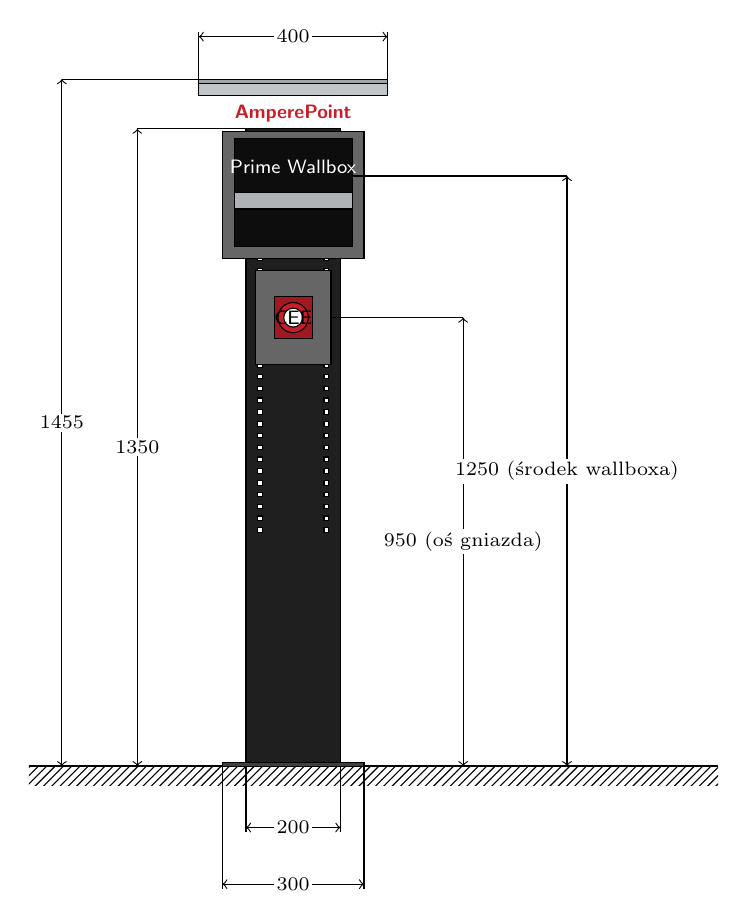
\begin{tikzpicture}[x=0.0060cm,y=0.0060cm]
% ---- WIDOK Z PRZODU, konfiguracja A ----
\fill[pattern=north east lines] (-560,-40) rectangle (900,0);
\draw[thick] (-560,0) -- (900,0);
\draw[fill=black!75] (-150,0) rectangle (150,8);
\draw[fill=black!88] (-100,8) rectangle (100,1350);
\foreach \y in {500,525,...,1300}{
  \draw[fill=white] (-74.75,\y-4.75) rectangle (-65.25,\y+4.75);
  \draw[fill=white] (65.25,\y-4.75) rectangle (74.75,\y+4.75);}
\draw[fill=black!60] (-150,1075) rectangle (150,1345);
\draw[fill=black!95] (-125,1100) rectangle (125,1330);
\draw[fill=apgray!60] (-125,1180) rectangle (125,1215);
\node[font=\scriptsize,white] at (0,1270) {\textsf{Prime Wallbox}};
\draw[fill=black!60] (-80,850) rectangle (80,1050);
\draw[fill=apred!80!black] (-40,905) rectangle (40,995);
\draw[fill=apred] (0,950) circle (32);
\draw[fill=white] (0,950) circle (20);
\node[font=\scriptsize] at (0,950) {\textsf{CEE}};
\draw[fill=apgray!45] (-200,1420) rectangle (200,1445);
\draw[fill=apgray!70] (-200,1445) rectangle (200,1455);
\node[font=\scriptsize,apred] at (0,1382) {\textsf{\textbf{AmperePoint}}};
\dimh{-100}{100}{-130}{200}
\dimh{-150}{150}{-250}{300}
\dimh{-200}{200}{1545}{400}
\dimv{-330}{0}{1350}{1350}
\dimv{-490}{0}{1455}{1455}
\dimv{360}{0}{950}{950 (oś gniazda)}
\dimv{580}{0}{1250}{1250 (środek wallboxa)}
\draw[thin] (-100,0) -- (-100,-140); \draw[thin] (100,0) -- (100,-140);
\draw[thin] (-150,0) -- (-150,-260); \draw[thin] (150,0) -- (150,-260);
\draw[thin] (-200,1455) -- (-200,1555); \draw[thin] (200,1455) -- (200,1555);
\draw[thin] (-330,1350) -- (-100,1350);
\draw[thin] (-490,1455) -- (-200,1455);
\draw[thin] (580,1250) -- (125,1250);
\draw[thin] (360,950) -- (80,950);
\end{tikzpicture}
\caption{AP-S1, widok z przodu --- konfiguracja A (wallbox Prime + gniazdo siłowe). Widoczne pasy
rastra montażowego (otwory kwadratowe co 25~mm).}
\label{fig:front}
\end{figure}

\begin{figure}[h]\centering
\begin{tikzpicture}[x=0.0060cm,y=0.0060cm]
% ---- WIDOK Z BOKU (prawy), konfiguracja A ----
\fill[pattern=north east lines] (-560,-40) rectangle (760,0);
\draw[thick] (-560,0) -- (760,0);
\draw[fill=black!75] (-125,0) rectangle (125,8);
\draw[fill=black!88] (-60,8) rectangle (60,1350);
% kanal kablowy (przerywana)
\draw[dashed,apred,thick] (0,-200) -- (0,600) -- (20,620) -- (20,900);
\draw[dashed,apred,thick] (20,940) -- (20,1200) -- (30,1215);
\node[font=\scriptsize,apred,anchor=west] at (150,-170) {\textsf{kabel zasilający z ziemi}};
\draw[thin,apred] (148,-170) -- (5,-185);
% szyna TH35 na 600
\draw[fill=apnavy!30] (-8,585) rectangle (8,615);
\node[font=\scriptsize,anchor=east,align=right] at (-100,600) {\textsf{szyna TH35}\\\textsf{(zabezpieczenia)}};
\draw[thin] (-98,600) -- (-8,600);
% wallbox na froncie (front = x=60)
\draw[fill=black!60] (60,1075) rectangle (72,1345);
\draw[fill=black!95] (72,1100) rectangle (212,1330);
\draw[fill=apgray!60] (72,1180) rectangle (212,1215);
% gniazdo CEE
\draw[fill=black!60] (60,850) rectangle (70,1050);
\draw[fill=apred!80!black] (70,905) rectangle (135,995);
\draw[fill=apred] (135,920) -- (168,935) -- (168,975) -- (135,985) -- cycle;
% daszek 350 w rzucie: od -60 (tyl) do 290 (przod); przod 1455, tyl 1381 (spadek 12 st do tylu)
\draw[fill=apgray!70] (-60,1381) -- (290,1455) -- (290,1441) -- (-60,1367) -- cycle;
\node[font=\scriptsize,anchor=west] at (330,1452) {\textsf{daszek, spadek $12^\circ$}};
\draw[thin] (328,1452) -- (240,1446);
% wsporniki daszka
\draw[fill=black!70] (-40,1350) -- (-40,1379) -- (40,1394) -- (40,1350) -- cycle;
% wymiary
\dimh{-60}{60}{-140}{120}
\dimh{-125}{125}{-260}{250}
\dimh{-60}{290}{1560}{350}
\dimh{60}{290}{560}{230 (wysunięcie)}
\draw[thin] (-60,0) -- (-60,-150); \draw[thin] (60,0) -- (60,-150);
\draw[thin] (-125,0) -- (-125,-270); \draw[thin] (125,0) -- (125,-270);
\draw[thin] (-60,1381) -- (-60,1550); \draw[thin] (290,1455) -- (290,1550);
\draw[thin] (60,560) -- (60,845); \draw[thin] (290,560) -- (290,1441);
\dimv{-320}{0}{1350}{1350}
\draw[thin] (-320,1350) -- (-60,1350);
\dimv{640}{0}{1455}{1455 (max)}
\draw[thin] (640,1455) -- (290,1455);
\node[font=\scriptsize,anchor=west,align=left] at (330,330) {\textsf{otwór rewizyjny}\\\textsf{$120\times250$ za płytą P2}};
\draw[thin] (328,330) -- (66,900);
\end{tikzpicture}
\caption{AP-S1, widok z boku. Czerwona linia przerywana --- trasa kabla: z ziemi, przez przepust
w płycie podstawy, kanałem wewnętrznym przez strefę zabezpieczeń do gniazda i wallboxa.}
\label{fig:bok}
\end{figure}

\begin{figure}[h]\centering
\begin{tikzpicture}[scale=0.022]
% ---- PRZEKROJ POZIOMY A-A ----
\draw[fill=black!15] (-100,-60) rectangle (100,60);
\draw[fill=white] (-97,-57) rectangle (97,57);
\draw[thick] (-100,30) -- (-90,30); \draw[thick] (-100,-30) -- (-90,-30);
\draw[thick] (100,30) -- (90,30); \draw[thick] (100,-30) -- (90,-30);
\foreach \x in {-70,70}{ \draw[fill=white] (\x-4.75,57) rectangle (\x+4.75,63);}
\foreach \x in {-70,70}{ \draw[fill=white] (\x-4.75,-63) rectangle (\x+4.75,-57);}
\draw[apnavy,thick] (-79,50) rectangle (-61,57);
\node[font=\scriptsize,apnavy,anchor=east,align=right] at (-125,42) {\textsf{nakrętka koszykowa M6}\\\textsf{wpinana od wewnątrz}};
\draw[thin,apnavy] (-123,42) -- (-79,52);
\draw[fill=black!40] (-80,63) rectangle (80,69);
\node[font=\scriptsize,anchor=west] at (115,85) {\textsf{płyta adapterowa (P1--P6), śruby M6}};
\draw[thin] (113,85) -- (60,67);
\draw[dashed,apred,thick] (-20,-40) rectangle (20,40);
\node[font=\scriptsize,apred] at (0,0) {\textsf{kanał}};
\draw[fill=apnavy!30] (-40,-54) rectangle (40,-47);
\node[font=\scriptsize,anchor=west] at (115,-70) {\textsf{szyna TH35 przy tylnej ścianie}};
\draw[thin] (113,-70) -- (40,-51);
\dimh{-100}{100}{-100}{200}
\dimv{145}{-60}{60}{120}
\draw[thin] (-100,-60) -- (-100,-105); \draw[thin] (100,-60) -- (100,-105);
\draw[thin] (100,-60) -- (150,-60); \draw[thin] (100,60) -- (150,60);
\node[font=\scriptsize] at (0,-85) {\textsf{blacha 3~mm}};
\end{tikzpicture}
\caption{Przekrój poziomy korpusu. Front (u góry) i tył identyczne --- stąd wersja DUO bez zmian
konstrukcyjnych. Płyty adapterowe kryją otwory rewizyjne.}
\label{fig:przekroj}
\end{figure}

\begin{figure}[h]\centering
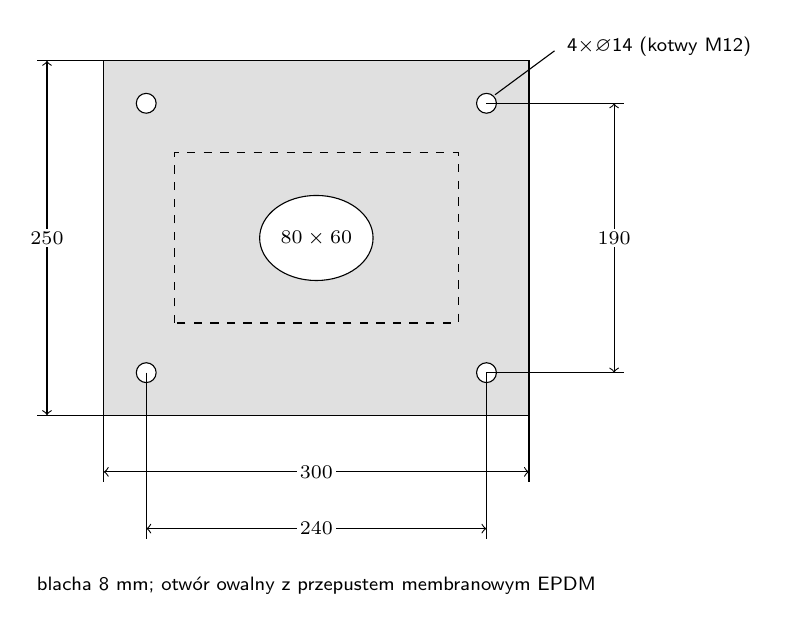
\begin{tikzpicture}[scale=0.018]
% ---- PLYTA PODSTAWY ----
\draw[fill=black!12] (-150,-125) rectangle (150,125);
\draw[dashed] (-100,-60) rectangle (100,60);
\draw[fill=white] (0,0) ellipse [x radius=40, y radius=30];
\node[font=\scriptsize] at (0,0) {\textsf{$80\times60$}};
\foreach \x in {-120,120}{\foreach \y in {-95,95}{
  \draw[fill=white] (\x,\y) circle (7);}}
\node[font=\scriptsize,anchor=west] at (170,135) {\textsf{4$\times\varnothing$14 (kotwy M12)}};
\draw[thin] (168,132) -- (126,101);
\dimh{-150}{150}{-165}{300}
\dimh{-120}{120}{-205}{240}
\dimv{-190}{-125}{125}{250}
\dimv{210}{-95}{95}{190}
\draw[thin] (-150,-125) -- (-150,-172); \draw[thin] (150,-125) -- (150,-172);
\draw[thin] (-120,-95) -- (-120,-212); \draw[thin] (120,-95) -- (120,-212);
\draw[thin] (-150,-125) -- (-197,-125); \draw[thin] (-150,125) -- (-197,125);
\draw[thin] (120,-95) -- (217,-95); \draw[thin] (120,95) -- (217,95);
\node[font=\scriptsize] at (0,-245) {\textsf{blacha 8~mm; otwór owalny z przepustem membranowym EPDM}};
\end{tikzpicture}
\caption{Płyta podstawy $300\times250\times8$~mm --- rzut z góry.}
\label{fig:podstawa}
\end{figure}

\begin{figure}[h]\centering
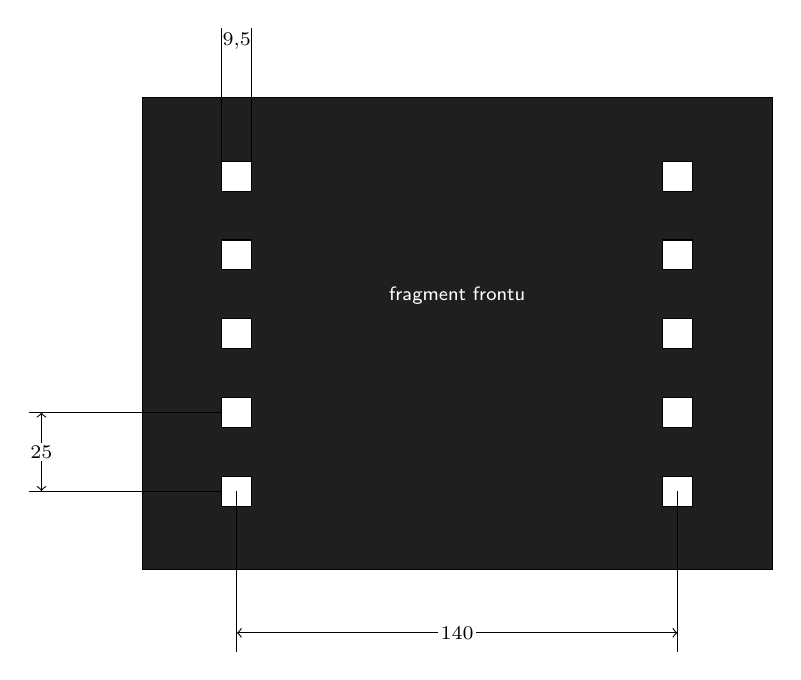
\begin{tikzpicture}[scale=0.040]
% ---- DETAL RASTRA ----
\draw[fill=black!88] (0,0) rectangle (200,150);
\foreach \y in {25,50,...,125}{
  \draw[fill=white] (30-4.75,\y-4.75) rectangle (30+4.75,\y+4.75);
  \draw[fill=white] (170-4.75,\y-4.75) rectangle (170+4.75,\y+4.75);}
\dimh{30}{170}{-20}{140}
\dimv{-32}{25}{50}{25}
\dimh{25.25}{34.75}{168}{9{,}5}
\draw[thin] (30,25) -- (30,-26); \draw[thin] (170,25) -- (170,-26);
\draw[thin] (25.25,129.75) -- (25.25,172); \draw[thin] (34.75,129.75) -- (34.75,172);
\draw[thin] (-36,25) -- (25,25); \draw[thin] (-36,50) -- (25,50);
\node[font=\scriptsize,white] at (100,87) {\textsf{fragment frontu}};
\end{tikzpicture}
\caption{Detal rastra montażowego: otwory kwadratowe $9{,}5\times9{,}5$~mm, podziałka pionowa 25~mm,
rozstaw pasów 140~mm --- standard nakrętek koszykowych M6 znany z szaf teleinformatycznych.}
\label{fig:raster}
\end{figure}

\begin{figure}[h]\centering
\begin{tikzpicture}[x=0.0058cm,y=0.0058cm]
% ---- ZESTAW DOPOSAZENIA AP-R1 na istniejacym slupku ----
\fill[pattern=north east lines] (-460,-40) rectangle (660,0);
\draw[thick] (-460,0) -- (660,0);
\draw[fill=black!75] (-110,0) rectangle (110,8);
\draw[fill=black!88] (-40,8) rectangle (40,1200);
\node[font=\scriptsize,white,rotate=90] at (0,300) {\textsf{istniejący profil}};
\foreach \y in {700,1150}{
  \draw[fill=apnavy!70] (-55,\y-15) rectangle (55,\y+15);
  \draw[fill=black!30] (-62,\y-8) rectangle (-55,\y+8);
  \draw[fill=black!30] (55,\y-8) rectangle (62,\y+8);}
\node[font=\scriptsize,anchor=east,align=right] at (-120,1150) {\textsf{obejma śrubowa M8}\\\textsf{(wkładka EPDM)}};
\draw[thin] (-118,1150) -- (-56,1150);
\node[font=\scriptsize,anchor=east] at (-120,700) {\textsf{obejma dolna}};
\draw[thin] (-118,700) -- (-56,700);
% daszek na gornej obejmie
\draw[fill=apgray!70] (-140,1230) -- (210,1298) -- (210,1283) -- (-140,1215) -- cycle;
\draw[fill=black!70] (-20,1200) -- (-20,1222) -- (20,1230) -- (20,1200) -- cycle;
\dimh{-140}{210}{1400}{350}
\draw[thin] (-140,1230) -- (-140,1390); \draw[thin] (210,1298) -- (210,1390);
% plyta osprzetowa na obejmach
\draw[fill=black!55] (55,640) rectangle (67,1165);
\draw[fill=black!40] (67,820) rectangle (79,1120);
\foreach \y in {845,870,...,1095}{ \draw[fill=white] (69,\y-4) rectangle (77,\y+4);}
\node[font=\scriptsize,anchor=west,align=left] at (250,1090) {\textsf{płyta osprzętowa z rastrem}\\\textsf{(gniazda bez wiercenia)}};
\draw[thin] (248,1090) -- (79,1010);
% gniazdo CEE na plycie
\draw[fill=apred!80!black] (79,900) rectangle (140,990);
\draw[fill=apred] (140,915) -- (170,928) -- (170,962) -- (140,977) -- cycle;
% maskownica pionowa kabla
\draw[fill=black!45] (-79,8) rectangle (-62,1135);
\node[font=\scriptsize,anchor=east,align=right] at (-150,320) {\textsf{maskownica kablowa}\\\textsf{C~$60\times40\times1{,}5$}};
\draw[thin] (-148,320) -- (-79,320);
% kabel z ziemi za maskownica
\draw[dashed,apred,thick] (-70,-160) -- (-70,1000) -- (0,1050);
\dimv{340}{0}{1200}{ok.~1200 (istn.)}
\draw[thin] (340,1200) -- (40,1200);
\dimv{490}{0}{1298}{1298}
\draw[thin] (490,1298) -- (210,1298);
\end{tikzpicture}
\caption{Zestaw doposażenia AP-R1 na istniejącym słupku: dwie obejmy śrubowe niosą daszek, pionową
maskownicę kabla (kabel z ziemi biegnie za nią) i płytę osprzętową z rastrem --- \textbf{zero
wierceń w profilu}. Wymiar obejm dobierany do zmierzonego profilu (zakres 60--100~mm).}
\label{fig:retrofit}
\end{figure}

\begin{figure}[h]\centering
\begin{tikzpicture}[x=0.0040cm,y=0.0040cm]
% ---- FUNDAMENTY: 3 warianty obok siebie ----
% A: kotwy
\begin{scope}[xshift=-4.6cm]
\fill[pattern=north east lines] (-260,-30) rectangle (260,0);
\draw[fill=black!20] (-260,-330) rectangle (260,-30);
\draw[thick] (-260,0) -- (260,0);
\draw[fill=black!75] (-150,0) rectangle (150,10);
\draw[fill=black!88] (-100,10) rectangle (100,330);
\foreach \x in {-120,120}{ \draw[fill=black!50] (\x-6,-160) rectangle (\x+6,10);}
\node[font=\scriptsize,align=center] at (0,-1000) {\textsf{\textbf{A.} kotwy wklejane}\\\textsf{M12$\times$160 w beton}};
\end{scope}
% B: prefabrykat
\begin{scope}
\fill[pattern=north east lines] (-260,-30) rectangle (260,0);
\draw[thick] (-260,0) -- (260,0);
\draw[fill=black!25] (-150,-800) rectangle (150,0);
\draw[fill=white] (-30,-800) rectangle (30,0);
\draw[fill=black!75] (-150,0) rectangle (150,10);
\draw[fill=black!88] (-100,10) rectangle (100,330);
\draw[dashed,apred,thick] (0,-760) -- (0,150);
\dimv{215}{-800}{0}{800}
\draw[thin] (215,-800) -- (150,-800); \draw[thin] (215,0) -- (150,0);
\node[font=\scriptsize,align=center] at (0,-1000) {\textsf{\textbf{B.} prefabrykat $300\times300\times800$}\\\textsf{z rurą $\varnothing$50 na kabel}};
\end{scope}
% C: sruba ziemna
\begin{scope}[xshift=4.6cm]
\fill[pattern=north east lines] (-260,-30) rectangle (260,0);
\draw[thick] (-260,0) -- (260,0);
\draw[fill=black!45] (-38,-100) rectangle (38,0);
\draw[fill=black!45] (-28,-865) -- (28,-865) -- (38,-100) -- (-38,-100) -- cycle;
\foreach \y in {-750,-650,-550,-450,-350,-250}{ \draw[thick] (-70,\y) -- (70,\y+55);}
\draw[fill=black!75] (-150,0) rectangle (150,10);
\draw[fill=black!88] (-100,10) rectangle (100,330);
\dimv{215}{-865}{0}{865}
\draw[thin] (215,-865) -- (28,-865); \draw[thin] (215,0) -- (150,0);
\node[font=\scriptsize,align=center] at (0,-1000) {\textsf{\textbf{C.} śruba ziemna $\varnothing$76$\times$865}\\\textsf{montaż bez betonu}};
\end{scope}
\end{tikzpicture}
\caption{Trzy warianty posadowienia AP-S1. W wariantach A i C kabel doprowadza się rurą osłonową
obok/przez oś słupka do otworu w płycie podstawy.}
\label{fig:fundamenty}
\end{figure}

\clearpage
\section{Lista materiałów (zestawienie elementów do wyceny)}
\begin{table}[h]\small
\caption{AP-S1 --- główne pozycje. Ceny do potwierdzenia u wykonawcy; kolumna ,,szacunek'' to rząd
wielkości przy serii 20--50 sztuk.}
\begin{tabular}{p{6.2cm}p{4.6cm}p{2.2cm}p{2.2cm}}
\toprule
Pozycja & Materiał / uwagi & Ilość & Szacunek\\
\midrule
Korpus (2 ceowniki gięte) & blacha DC01/S235JR 3~mm, cięcie laserowe + gięcie + spawanie & 1 kpl & 180--260~zł\\
Płyta podstawy & blacha 8~mm, otwory laserowo & 1 szt. & 40--60~zł\\
Daszek & blacha 2~mm gięta, RAL~9006 & 1 szt. & 35--55~zł\\
Płyty adapterowe P1--P6 & blacha 3~mm, z dławikami & wg konfig. & 15--30~zł/szt.\\
Ocynk + malowanie proszkowe & RAL~9005 struktura & kpl & 120--180~zł\\
Nitonakrętki M6 + nakrętki koszykowe M6 + śruby M6 A2 & stal nierdzewna A2 & ok. 40 szt. & 30--45~zł\\
Przepust membranowy EPDM + dławiki M32 & --- & kpl & 20--35~zł\\
Szyna TH35 160~mm + złączki N/PE & --- & 1 kpl & 25--40~zł\\
Uszczelki EPDM samoprzylepne & pod płyty i daszek & kpl & 10--15~zł\\
\midrule
\multicolumn{3}{r}{\textbf{Razem koszt wytworzenia (bez osprzętu elektrycznego):}} & \textbf{ok.~475--720~zł}\\
\multicolumn{3}{r}{Proponowana cena detaliczna (daszek i raster w standardzie):} & 999--1199~zł\\
\bottomrule
\end{tabular}
\end{table}

\begin{table}[h]\small
\caption{AP-R1 (zestaw doposażenia) --- główne pozycje.}
\begin{tabular}{p{6.2cm}p{4.6cm}p{2.2cm}p{2.2cm}}
\toprule
Pozycja & Materiał / uwagi & Ilość & Szacunek\\
\midrule
Obejmy śrubowe z wkładką EPDM & płaskownik 40$\times$5, śruby M8 A2, zakres 60--100~mm & 2 szt. & 40--60~zł\\
Daszek $350\times300$ & blacha 2~mm, RAL~9006 & 1 szt. & 30--50~zł\\
Maskownica kablowa & ceownik $60\times40\times1{,}5$~mm, dł. 1200~mm & 1 szt. & 25--40~zł\\
Płyta osprzętowa z rastrem & blacha 3~mm, $200\times300$ & 1 szt. & 20--35~zł\\
Malowanie proszkowe + złączki & RAL~9005/9006 & kpl & 40--60~zł\\
\midrule
\multicolumn{3}{r}{\textbf{Razem koszt wytworzenia:}} & \textbf{ok.~155--245~zł}\\
\multicolumn{3}{r}{Proponowana cena detaliczna zestawu:} & 349--449~zł\\
\bottomrule
\end{tabular}
\end{table}

\section{Przewagi nad konkurencją i innowacje własne}
\begin{enumerate}
\item \textbf{Raster nakrętek koszykowych} --- montaż gniazd, uchwytów i ładowarek bez jednego
wiercenia, na dowolnej wysokości co 25~mm, w pełni odwracalny. Nikt na rynku słupków EV tego nie
stosuje (Platinet daje jeden adapter, reszta --- otwory pod konkretny model).
\item \textbf{Daszek w standardzie} --- u konkurencji brak (Green Wallbox, Green Cell) albo płatna
opcja (Wallbox Eiffel).
\item \textbf{Kabel z ziemi w 100\% wewnątrz} + fabryczny przepust w płycie podstawy i otwory
rewizyjne za płytami --- podłączenie gniazda ręką, bez demontażu słupka.
\item \textbf{Strefa zabezpieczeń TH35 w słupku} --- wyłącznik różnicowoprądowy przy stanowisku,
opcja licznika (rozliczanie najemcy/pracownika). W segmencie do 1500~zł nie oferuje tego nikt.
\item \textbf{Gniazda jako element systemu} --- płyty pod gniazdo siłowe i Dr.~Storm wprost pod
model sprzedaży AMPERE POINT (ładowarka przenośna + gniazdo przy stanowisku).
\item \textbf{Wersja DUO bez zmian konstrukcyjnych} (identyczny raster z tyłu).
\item \textbf{Trzy warianty posadowienia}, w tym śruba ziemna --- montaż w pół godziny bez betonu,
odwracalny (klient wynajmujący dom); prefabrykat jako akcesorium wzorem konkurencji.
\item \textbf{Zestaw doposażenia AP-R1} --- monetyzacja już sprzedanych/ustawionych słupków
(showroom też), spójny wizualnie z nowym produktem.
\item \textbf{Styl marki}: czerń strukturalna + srebrny daszek + czerwone logo (opcjonalnie
podświetlane listwą LED) --- słupek rozpoznawalny jak Q11.
\end{enumerate}

\section{Bezpieczeństwo i zgodność --- uwagi do projektu elektrycznego}
Słupek jest konstrukcją mechaniczną; obwody zasilające projektuje i wykonuje elektryk z uprawnieniami.
Do pilnowania na etapie wdrożenia:
\begin{itemize}
\item gniazda i osprzęt na zewnątrz min. IP44 (siłowe wg PN-EN 60309), wysokość gniazd w przedziale
0{,}5--1{,}5~m --- projekt: 950/1000~mm;
\item obwody ładowania wg HD 60364-7-722 (m.in. osobny obwód na punkt, wyłącznik różnicowoprądowy
typu A z detekcją prądu stałego 6~mA albo typu B --- zależnie od ładowarki);
\item ciągłość PE wszystkich części metalowych (korpus, daszek, płyty) --- przewidziane linki
wyrównawcze i śruba PE M8;
\item przekroje i zabezpieczenia dobrane do mocy (16~A/11~kW lub 32~A/22~kW) i długości linii
zasilającej z budynku;
\item strefa zabezpieczeń w słupku jako rozdzielnica wg PN-EN 61439 (gotowa obudowa IP65 na TH35
załatwia temat certyfikacyjny).
\end{itemize}

\section{Dalsze kroki}
\begin{enumerate}
\item Zmierzyć dokładny przekrój profili obecnych słupków (do produkcji obejm AP-R1; zakładany
zakres 60--100~mm).
\item Zdecydować o nazwie handlowej i ostatecznej kolorystyce daszka (srebrny RAL~9006 vs czerń).
\item Zlecić wykonanie plików DXF (rozwinięcia blach) na bazie tego dokumentu i wycenę u 2--3
wykonawców (cięcie laserowe + gięcie + spawanie + ocynk + proszek), seria próbna: 2 szt. AP-S1
(po jednej na konfigurację) + 2 kpl. AP-R1.
\item Prototyp: montaż obu konfiguracji, test wodny daszka i przepustów, poprawki, sesja zdjęciowa
do sklepu.
\item Karta produktu + instrukcja montażu (wzorem karty AMP-BOX).
\end{enumerate}

\section*{Źródła (research, dostęp: 12.07.2026)}
\begin{itemize}\small
\item AMPERE POINT --- sklep i produkty: \url{https://www.amperepoint.pl/} (AMP-BOX ze słupkiem 999~zł,
Dr.~Storm 179~zł, Prime Wallbox, seria Q).
\item Platinet --- uniwersalny słupek z daszkiem, 1100~zł, wys. 130~cm, profil 8$\times$8~cm:
\url{https://sklep.platinet.pl/pl/p/Uniwersalny-slupek-montazowy-do-ladowarek-EV-typu-Wallbox-z-daszkiem/214763}
\item Green Cell GC EV Stand (EVSTND01), ok. 480~zł: \url{https://swiatbaterii.pl/akcesoria-ev/36974-green-cell-slupek-montazowy-gc-ev-stand-do-stacji-ladowania-samochodow-elektrycznych-wallbox.html}
\item Green Wallbox --- słupki 649--979~zł, fundament 399~zł:
\url{https://greenwallbox.pl/collections/slupek-do-stacji-ladowania}
\item Wallbox Eiffel Basic, ok. 450--550~USD, osłona przeciwdeszczowa ok. 80~USD:
\url{https://support.wallbox.com/en/knowledge-base/eiffel-pedestal-accessory-overview/},
\url{https://shop.wallbox.com/products/eiffel-basic-pedestal}
\item Enelion Vertica (moduły 5000--6650~zł): \url{https://enelion.com/pl/product/vertica/},
\url{https://sklep.polska-energia.com/98-stacje-ladowania-pojazdow}
\item Tuneon Design (DE) --- stele 147--165~EUR, warianty z osłoną przeciwdeszczową:
\url{https://www.tuneon-design.com/en/wallbox-pillars/}
\item KEBA KC-P30 Pedestal (stal nierdzewna): \url{https://www.store-charge.com/Keba-KC-P30-Pedestal-Single-stainless-steel/KE-03-02}
\item easee Base pedestal: \url{https://www.electricpoint.com/easee-base-ground-mount.html}
\end{itemize}

\vspace{0.6em}
\noindent\textit{Wymagane w ramach projektu, do wykonania po akceptacji koncepcji: pliki DXF
rozwinięć blach, dokumentacja warsztatowa (tolerancje, spoiny), instrukcja montażu i karta produktu.}

\end{document}
